\chapter{L�gica Fuzzy}

Esta se��o tem como fun��o descrever o que � a l�gica fuzzy, em que teorias
foi baseada, onde pode ser utilizada e quais s�o suas vantagens e desvantagens.

A l�gica fuzzy � baseada no trabalho de Lofti Zadeh, que prop�s a teoria de conjuntos
fuzzy em 1965\cite{FUZZYLOGIC}. Na teoria cl�ssica de conjuntos, um elemento tem seu
grau de pertin�ncia ao conjunto representado por uma vari�vel booleana, ou seja, ou o elemento
pertence ao conjunto ou n�o pertence. Num conjunto fuzzy, no entanto, um elemento tem seu grau
de pertin�ncia representado por um valor real no intervalo [0, 1].

Uma aplica�ao b�sica da l�gica fuzzy � a classifica��o de uma vari�vel cont�nua. Por exemplo, se fosse necess�rio classificar um valor de temperatura, poderia ser utilizado um conjunto fuzzy com as vari�veis
FRIO, MORNO e QUENTE. Para saber a classifica��o de certo valor de temperatura, poderia ser utilizado algo
como o que est� representado na figura \ref{fig:fuzzyclasses}.

\begin{figure}[!htb]
    \centering
    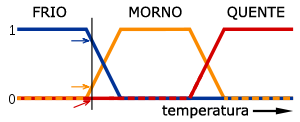
\includegraphics{./figs/fuzzyclasses.png}
    \caption[Classifica��o Fuzzy]{Classifica��o de valores de temperatura utilizando l�gica fuzzy.}
    \fonte{\cite{FUZZYLOGIC}}
    \label{fig:fuzzyclasses}
\end{figure} 